\documentclass[twoside]{book}

% Packages required by doxygen
\usepackage{fixltx2e}
\usepackage{calc}
\usepackage{doxygen}
\usepackage[export]{adjustbox} % also loads graphicx
\usepackage{graphicx}
\usepackage[utf8]{inputenc}
\usepackage{makeidx}
\usepackage{multicol}
\usepackage{multirow}
\PassOptionsToPackage{warn}{textcomp}
\usepackage{textcomp}
\usepackage[nointegrals]{wasysym}
\usepackage[table]{xcolor}

% Font selection
\usepackage[T1]{fontenc}
\usepackage[scaled=.90]{helvet}
\usepackage{courier}
\usepackage{amssymb}
\usepackage{sectsty}
\renewcommand{\familydefault}{\sfdefault}
\allsectionsfont{%
  \fontseries{bc}\selectfont%
  \color{darkgray}%
}
\renewcommand{\DoxyLabelFont}{%
  \fontseries{bc}\selectfont%
  \color{darkgray}%
}
\newcommand{\+}{\discretionary{\mbox{\scriptsize$\hookleftarrow$}}{}{}}

% Page & text layout
\usepackage{geometry}
\geometry{%
  a4paper,%
  top=2.5cm,%
  bottom=2.5cm,%
  left=2.5cm,%
  right=2.5cm%
}
\tolerance=750
\hfuzz=15pt
\hbadness=750
\setlength{\emergencystretch}{15pt}
\setlength{\parindent}{0cm}
\setlength{\parskip}{3ex plus 2ex minus 2ex}
\makeatletter
\renewcommand{\paragraph}{%
  \@startsection{paragraph}{4}{0ex}{-1.0ex}{1.0ex}{%
    \normalfont\normalsize\bfseries\SS@parafont%
  }%
}
\renewcommand{\subparagraph}{%
  \@startsection{subparagraph}{5}{0ex}{-1.0ex}{1.0ex}{%
    \normalfont\normalsize\bfseries\SS@subparafont%
  }%
}
\makeatother

% Headers & footers
\usepackage{fancyhdr}
\pagestyle{fancyplain}
\fancyhead[LE]{\fancyplain{}{\bfseries\thepage}}
\fancyhead[CE]{\fancyplain{}{}}
\fancyhead[RE]{\fancyplain{}{\bfseries\leftmark}}
\fancyhead[LO]{\fancyplain{}{\bfseries\rightmark}}
\fancyhead[CO]{\fancyplain{}{}}
\fancyhead[RO]{\fancyplain{}{\bfseries\thepage}}
\fancyfoot[LE]{\fancyplain{}{}}
\fancyfoot[CE]{\fancyplain{}{}}
\fancyfoot[RE]{\fancyplain{}{\bfseries\scriptsize Generated by Doxygen }}
\fancyfoot[LO]{\fancyplain{}{\bfseries\scriptsize Generated by Doxygen }}
\fancyfoot[CO]{\fancyplain{}{}}
\fancyfoot[RO]{\fancyplain{}{}}
\renewcommand{\footrulewidth}{0.4pt}
\renewcommand{\chaptermark}[1]{%
  \markboth{#1}{}%
}
\renewcommand{\sectionmark}[1]{%
  \markright{\thesection\ #1}%
}

% Indices & bibliography
\usepackage{natbib}
\usepackage[titles]{tocloft}
\setcounter{tocdepth}{3}
\setcounter{secnumdepth}{5}
\makeindex

% Hyperlinks (required, but should be loaded last)
\usepackage{ifpdf}
\ifpdf
  \usepackage[pdftex,pagebackref=true]{hyperref}
\else
  \usepackage[ps2pdf,pagebackref=true]{hyperref}
\fi
\hypersetup{%
  colorlinks=true,%
  linkcolor=blue,%
  citecolor=blue,%
  unicode%
}

% Custom commands
\newcommand{\clearemptydoublepage}{%
  \newpage{\pagestyle{empty}\cleardoublepage}%
}

\usepackage{caption}
\captionsetup{labelsep=space,justification=centering,font={bf},singlelinecheck=off,skip=4pt,position=top}

%===== C O N T E N T S =====

\begin{document}

% Titlepage & ToC
\hypersetup{pageanchor=false,
             bookmarksnumbered=true,
             pdfencoding=unicode
            }
\pagenumbering{alph}
\begin{titlepage}
\vspace*{7cm}
\begin{center}%
{\Large My Project }\\
\vspace*{1cm}
{\large Generated by Doxygen 1.8.13}\\
\end{center}
\end{titlepage}
\clearemptydoublepage
\pagenumbering{roman}
\tableofcontents
\clearemptydoublepage
\pagenumbering{arabic}
\hypersetup{pageanchor=true}

%--- Begin generated contents ---
\chapter{File Index}
\section{File List}
Here is a list of all documented files with brief descriptions\+:\begin{DoxyCompactList}
\item\contentsline{section}{\hyperlink{exit__codes_8h}{exit\+\_\+codes.\+h} \\*Заголовочный файл с описанием ошибок }{\pageref{exit__codes_8h}}{}
\item\contentsline{section}{\hyperlink{main_8c}{main.\+c} \\*Функция main }{\pageref{main_8c}}{}
\item\contentsline{section}{\hyperlink{str__processing_8c}{str\+\_\+processing.\+c} \\*Код функций, обрабатывающих строки }{\pageref{str__processing_8c}}{}
\item\contentsline{section}{\hyperlink{str__processing_8h}{str\+\_\+processing.\+h} \\*Заголовочный файл с описанием функций, обрабатывающих строки }{\pageref{str__processing_8h}}{}
\end{DoxyCompactList}

\chapter{File Documentation}
\hypertarget{exit__codes_8h}{}\section{exit\+\_\+codes.\+h File Reference}
\label{exit__codes_8h}\index{exit\+\_\+codes.\+h@{exit\+\_\+codes.\+h}}


Заголовочный файл с описанием ошибок  


This graph shows which files directly or indirectly include this file\+:
\nopagebreak
\begin{figure}[H]
\begin{center}
\leavevmode
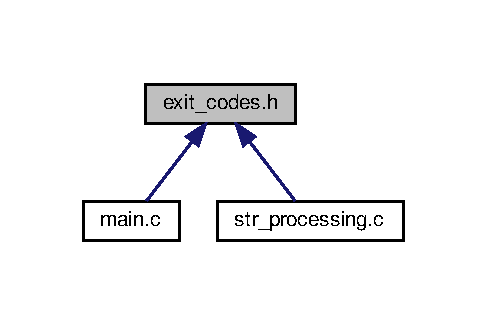
\includegraphics[width=234pt]{exit__codes_8h__dep__incl}
\end{center}
\end{figure}
\subsection*{Macros}
\begin{DoxyCompactItemize}
\item 
\mbox{\Hypertarget{exit__codes_8h_aa90cac659d18e8ef6294c7ae337f6b58}\label{exit__codes_8h_aa90cac659d18e8ef6294c7ae337f6b58}} 
\#define {\bfseries S\+U\+C\+C\+E\+SS}~0
\item 
\mbox{\Hypertarget{exit__codes_8h_ac41734365e76e2fcab439c31c28ea28c}\label{exit__codes_8h_ac41734365e76e2fcab439c31c28ea28c}} 
\#define {\bfseries R\+E\+A\+D\+\_\+\+E\+R\+R\+OR}~1
\item 
\mbox{\Hypertarget{exit__codes_8h_ae2a67d095d092a72f540301e7ac4f7cb}\label{exit__codes_8h_ae2a67d095d092a72f540301e7ac4f7cb}} 
\#define {\bfseries R\+E\+A\+D\+\_\+\+E\+M\+P\+TY}~2
\item 
\mbox{\Hypertarget{exit__codes_8h_aef2d15d47db11c4c81291c403247b189}\label{exit__codes_8h_aef2d15d47db11c4c81291c403247b189}} 
\#define {\bfseries S\+Y\+M\+B\+\_\+\+E\+R\+R\+OR}~3
\item 
\mbox{\Hypertarget{exit__codes_8h_a7f62d8d6f050391f0f3e6058867c4cfd}\label{exit__codes_8h_a7f62d8d6f050391f0f3e6058867c4cfd}} 
\#define {\bfseries W\+R\+I\+T\+E\+\_\+\+E\+R\+R\+OR}~4
\end{DoxyCompactItemize}


\subsection{Detailed Description}
Заголовочный файл с описанием ошибок 

Данный файл содержит в себе коды рассматриваемых ошибок, используемых в программе 
\hypertarget{main_8c}{}\section{main.\+c File Reference}
\label{main_8c}\index{main.\+c@{main.\+c}}


Функция main.  


{\ttfamily \#include $<$stdio.\+h$>$}\newline
{\ttfamily \#include $<$stdlib.\+h$>$}\newline
{\ttfamily \#include $<$string.\+h$>$}\newline
{\ttfamily \#include \char`\"{}exit\+\_\+codes.\+h\char`\"{}}\newline
{\ttfamily \#include \char`\"{}str\+\_\+processing.\+h\char`\"{}}\newline
Include dependency graph for main.\+c\+:\nopagebreak
\begin{figure}[H]
\begin{center}
\leavevmode
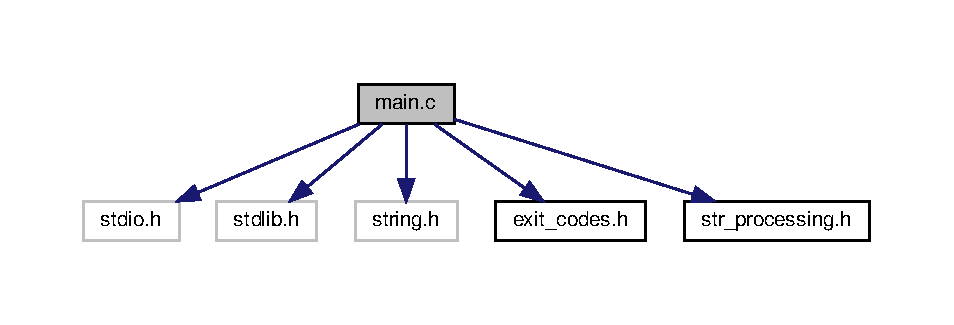
\includegraphics[width=350pt]{main_8c__incl}
\end{center}
\end{figure}
\subsection*{Macros}
\begin{DoxyCompactItemize}
\item 
\mbox{\Hypertarget{main_8c_a8f80f888c30735ca5629ee3d25f37694}\label{main_8c_a8f80f888c30735ca5629ee3d25f37694}} 
\#define {\bfseries F\+I\+L\+E\+\_\+\+T\+O\+\_\+\+R\+E\+AD}~\char`\"{}read.\+txt\char`\"{}
\item 
\mbox{\Hypertarget{main_8c_a89ff6d1018bdfd28bdc5bdcb2fe925d4}\label{main_8c_a89ff6d1018bdfd28bdc5bdcb2fe925d4}} 
\#define {\bfseries F\+I\+L\+E\+\_\+\+T\+O\+\_\+\+W\+R\+I\+TE}~\char`\"{}write.\+txt\char`\"{}
\end{DoxyCompactItemize}
\subsection*{Functions}
\begin{DoxyCompactItemize}
\item 
int \hyperlink{main_8c_a840291bc02cba5474a4cb46a9b9566fe}{main} (void)
\end{DoxyCompactItemize}


\subsection{Detailed Description}
Функция main. 

Функция включает в себя работу с входным файлом и создает выходной, куда записывает данные 

\subsection{Function Documentation}
\mbox{\Hypertarget{main_8c_a840291bc02cba5474a4cb46a9b9566fe}\label{main_8c_a840291bc02cba5474a4cb46a9b9566fe}} 
\index{main.\+c@{main.\+c}!main@{main}}
\index{main@{main}!main.\+c@{main.\+c}}
\subsubsection{\texorpdfstring{main()}{main()}}
{\footnotesize\ttfamily int main (\begin{DoxyParamCaption}\item[{void}]{ }\end{DoxyParamCaption})}

Содержит обработку входного файла\+: его открытие и проверку на корректность


\begin{DoxyCode}
FILE *fr = fopen(FILE\_TO\_READ, \textcolor{stringliteral}{"r"});
\textcolor{keywordflow}{if} (!fr)
\{
    printf(\textcolor{stringliteral}{"The file to read does not exist.\(\backslash\)n"});
    exit\_code = READ\_ERROR;
\}
\end{DoxyCode}


Обработка строки в цикле\+: ее перевод(вызов необходимых функций) и запись в выходной файл


\begin{DoxyCode}
hec\_number = \hyperlink{str__processing_8c_a9e35d52c5c113b3c4cd685ead752d551}{translate}(bin\_number);
\hyperlink{str__processing_8c_a7dbe1ec23bd7aeafc02add2088b28aae}{inverse}(&hec\_number);
fwrite(hec\_number, strlen(hec\_number), 1, fw);
\end{DoxyCode}

\hypertarget{str__processing_8c}{}\section{str\+\_\+processing.\+c File Reference}
\label{str__processing_8c}\index{str\+\_\+processing.\+c@{str\+\_\+processing.\+c}}


Код функций, обрабатывающих строки  


{\ttfamily \#include $<$stdio.\+h$>$}\newline
{\ttfamily \#include $<$stdlib.\+h$>$}\newline
{\ttfamily \#include $<$string.\+h$>$}\newline
{\ttfamily \#include \char`\"{}exit\+\_\+codes.\+h\char`\"{}}\newline
{\ttfamily \#include \char`\"{}str\+\_\+processing.\+h\char`\"{}}\newline
Include dependency graph for str\+\_\+processing.\+c\+:\nopagebreak
\begin{figure}[H]
\begin{center}
\leavevmode
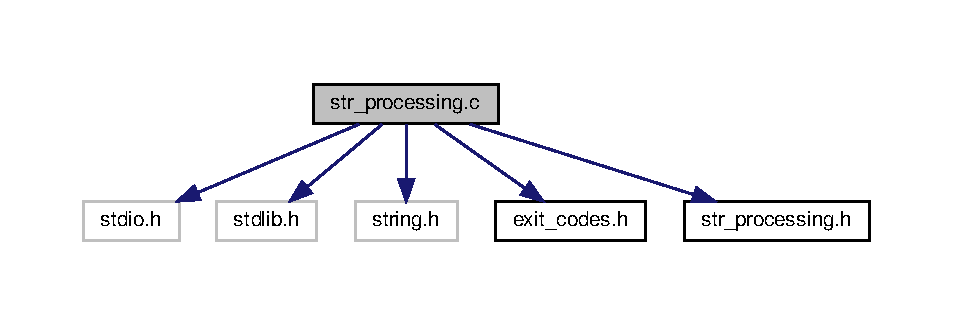
\includegraphics[width=350pt]{str__processing_8c__incl}
\end{center}
\end{figure}
\subsection*{Functions}
\begin{DoxyCompactItemize}
\item 
char $\ast$ \hyperlink{str__processing_8c_a469a334710c19e2d621acc940fe8fb31}{get\+\_\+string} (F\+I\+LE $\ast$f)
\item 
int \hyperlink{str__processing_8c_a50eac7ea4d5c8946c22c22039a85925b}{correct\+\_\+input} (char $\ast$str)
\item 
char $\ast$ \hyperlink{str__processing_8c_a9e35d52c5c113b3c4cd685ead752d551}{translate} (char $\ast$number)
\item 
void \hyperlink{str__processing_8c_a7dbe1ec23bd7aeafc02add2088b28aae}{inverse} (char $\ast$$\ast$string)
\end{DoxyCompactItemize}


\subsection{Detailed Description}
Код функций, обрабатывающих строки 

Данный файл содержит функции, используемые при переводе числа из одной СС в другую 

\subsection{Function Documentation}
\mbox{\Hypertarget{str__processing_8c_a50eac7ea4d5c8946c22c22039a85925b}\label{str__processing_8c_a50eac7ea4d5c8946c22c22039a85925b}} 
\index{str\+\_\+processing.\+c@{str\+\_\+processing.\+c}!correct\+\_\+input@{correct\+\_\+input}}
\index{correct\+\_\+input@{correct\+\_\+input}!str\+\_\+processing.\+c@{str\+\_\+processing.\+c}}
\subsubsection{\texorpdfstring{correct\+\_\+input()}{correct\_input()}}
{\footnotesize\ttfamily int correct\+\_\+input (\begin{DoxyParamCaption}\item[{char $\ast$}]{str }\end{DoxyParamCaption})}

Проверка строки на корректность записи 
\begin{DoxyParams}[1]{Parameters}
\mbox{\tt out}  & {\em int} & Код ошибки \\
\hline
\mbox{\tt in}  & {\em char$\ast$} & Строка \\
\hline
\end{DoxyParams}
\mbox{\Hypertarget{str__processing_8c_a469a334710c19e2d621acc940fe8fb31}\label{str__processing_8c_a469a334710c19e2d621acc940fe8fb31}} 
\index{str\+\_\+processing.\+c@{str\+\_\+processing.\+c}!get\+\_\+string@{get\+\_\+string}}
\index{get\+\_\+string@{get\+\_\+string}!str\+\_\+processing.\+c@{str\+\_\+processing.\+c}}
\subsubsection{\texorpdfstring{get\+\_\+string()}{get\_string()}}
{\footnotesize\ttfamily char$\ast$ get\+\_\+string (\begin{DoxyParamCaption}\item[{F\+I\+LE $\ast$}]{f }\end{DoxyParamCaption})}

Считывает посимвольно строку из файла 
\begin{DoxyParams}[1]{Parameters}
\mbox{\tt out}  & {\em char$\ast$} & Строка \\
\hline
\mbox{\tt in}  & {\em F\+I\+L\+E$\ast$} & Файловый указатель \\
\hline
\end{DoxyParams}
\mbox{\Hypertarget{str__processing_8c_a7dbe1ec23bd7aeafc02add2088b28aae}\label{str__processing_8c_a7dbe1ec23bd7aeafc02add2088b28aae}} 
\index{str\+\_\+processing.\+c@{str\+\_\+processing.\+c}!inverse@{inverse}}
\index{inverse@{inverse}!str\+\_\+processing.\+c@{str\+\_\+processing.\+c}}
\subsubsection{\texorpdfstring{inverse()}{inverse()}}
{\footnotesize\ttfamily void inverse (\begin{DoxyParamCaption}\item[{char $\ast$$\ast$}]{string }\end{DoxyParamCaption})}

Разворот строки 
\begin{DoxyParams}[1]{Parameters}
\mbox{\tt in}  & {\em char$\ast$} & Указатель на строку \\
\hline
\end{DoxyParams}
\mbox{\Hypertarget{str__processing_8c_a9e35d52c5c113b3c4cd685ead752d551}\label{str__processing_8c_a9e35d52c5c113b3c4cd685ead752d551}} 
\index{str\+\_\+processing.\+c@{str\+\_\+processing.\+c}!translate@{translate}}
\index{translate@{translate}!str\+\_\+processing.\+c@{str\+\_\+processing.\+c}}
\subsubsection{\texorpdfstring{translate()}{translate()}}
{\footnotesize\ttfamily char$\ast$ translate (\begin{DoxyParamCaption}\item[{char $\ast$}]{number }\end{DoxyParamCaption})}

Перевод числа из 2-\/чной СС в 16-\/ричную 
\begin{DoxyParams}{Parameters}
{\em str} & Строка, куда записано исходное число \\
\hline
\end{DoxyParams}
\begin{DoxyReturn}{Returns}
Строку в 16-\/ричной системе счисления 
\end{DoxyReturn}

\hypertarget{str__processing_8h}{}\section{str\+\_\+processing.\+h File Reference}
\label{str__processing_8h}\index{str\+\_\+processing.\+h@{str\+\_\+processing.\+h}}


Заголовочный файл с описанием функций, обрабатывающих строки  


This graph shows which files directly or indirectly include this file\+:
\nopagebreak
\begin{figure}[H]
\begin{center}
\leavevmode
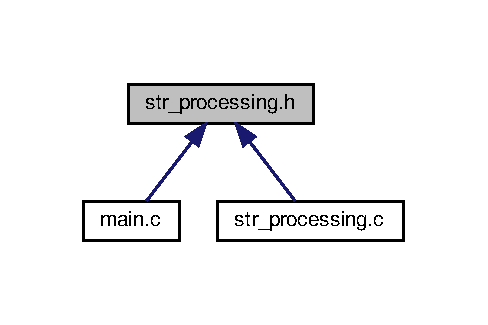
\includegraphics[width=234pt]{str__processing_8h__dep__incl}
\end{center}
\end{figure}
\subsection*{Functions}
\begin{DoxyCompactItemize}
\item 
char $\ast$ \hyperlink{str__processing_8h_a469a334710c19e2d621acc940fe8fb31}{get\+\_\+string} (F\+I\+LE $\ast$f)
\item 
int \hyperlink{str__processing_8h_a50eac7ea4d5c8946c22c22039a85925b}{correct\+\_\+input} (char $\ast$str)
\item 
char $\ast$ \hyperlink{str__processing_8h_a9e35d52c5c113b3c4cd685ead752d551}{translate} (char $\ast$number)
\item 
void \hyperlink{str__processing_8h_a7dbe1ec23bd7aeafc02add2088b28aae}{inverse} (char $\ast$$\ast$string)
\end{DoxyCompactItemize}


\subsection{Detailed Description}
Заголовочный файл с описанием функций, обрабатывающих строки 

Данный файл содержит функции, используемые при переводе числа из одной СС в другую 

\subsection{Function Documentation}
\mbox{\Hypertarget{str__processing_8h_a50eac7ea4d5c8946c22c22039a85925b}\label{str__processing_8h_a50eac7ea4d5c8946c22c22039a85925b}} 
\index{str\+\_\+processing.\+h@{str\+\_\+processing.\+h}!correct\+\_\+input@{correct\+\_\+input}}
\index{correct\+\_\+input@{correct\+\_\+input}!str\+\_\+processing.\+h@{str\+\_\+processing.\+h}}
\subsubsection{\texorpdfstring{correct\+\_\+input()}{correct\_input()}}
{\footnotesize\ttfamily int correct\+\_\+input (\begin{DoxyParamCaption}\item[{char $\ast$}]{str }\end{DoxyParamCaption})}

Проверка строки на корректность записи 
\begin{DoxyParams}[1]{Parameters}
\mbox{\tt out}  & {\em int} & Код ошибки \\
\hline
\mbox{\tt in}  & {\em char$\ast$} & Строка \\
\hline
\end{DoxyParams}
\mbox{\Hypertarget{str__processing_8h_a469a334710c19e2d621acc940fe8fb31}\label{str__processing_8h_a469a334710c19e2d621acc940fe8fb31}} 
\index{str\+\_\+processing.\+h@{str\+\_\+processing.\+h}!get\+\_\+string@{get\+\_\+string}}
\index{get\+\_\+string@{get\+\_\+string}!str\+\_\+processing.\+h@{str\+\_\+processing.\+h}}
\subsubsection{\texorpdfstring{get\+\_\+string()}{get\_string()}}
{\footnotesize\ttfamily char$\ast$ get\+\_\+string (\begin{DoxyParamCaption}\item[{F\+I\+LE $\ast$}]{f }\end{DoxyParamCaption})}

Считывает посимвольно строку из файла 
\begin{DoxyParams}[1]{Parameters}
\mbox{\tt out}  & {\em char$\ast$} & Строка \\
\hline
\mbox{\tt in}  & {\em F\+I\+L\+E$\ast$} & Файловый указатель \\
\hline
\end{DoxyParams}
\mbox{\Hypertarget{str__processing_8h_a7dbe1ec23bd7aeafc02add2088b28aae}\label{str__processing_8h_a7dbe1ec23bd7aeafc02add2088b28aae}} 
\index{str\+\_\+processing.\+h@{str\+\_\+processing.\+h}!inverse@{inverse}}
\index{inverse@{inverse}!str\+\_\+processing.\+h@{str\+\_\+processing.\+h}}
\subsubsection{\texorpdfstring{inverse()}{inverse()}}
{\footnotesize\ttfamily void inverse (\begin{DoxyParamCaption}\item[{char $\ast$$\ast$}]{string }\end{DoxyParamCaption})}

Разворот строки 
\begin{DoxyParams}[1]{Parameters}
\mbox{\tt in}  & {\em char$\ast$} & Указатель на строку \\
\hline
\end{DoxyParams}
\mbox{\Hypertarget{str__processing_8h_a9e35d52c5c113b3c4cd685ead752d551}\label{str__processing_8h_a9e35d52c5c113b3c4cd685ead752d551}} 
\index{str\+\_\+processing.\+h@{str\+\_\+processing.\+h}!translate@{translate}}
\index{translate@{translate}!str\+\_\+processing.\+h@{str\+\_\+processing.\+h}}
\subsubsection{\texorpdfstring{translate()}{translate()}}
{\footnotesize\ttfamily char$\ast$ translate (\begin{DoxyParamCaption}\item[{char $\ast$}]{number }\end{DoxyParamCaption})}

Перевод числа из 2-\/чной СС в 16-\/ричную 
\begin{DoxyParams}{Parameters}
{\em str} & Строка, куда записано исходное число \\
\hline
\end{DoxyParams}
\begin{DoxyReturn}{Returns}
Строку в 16-\/ричной системе счисления 
\end{DoxyReturn}

%--- End generated contents ---

% Index
\backmatter
\newpage
\phantomsection
\clearemptydoublepage
\addcontentsline{toc}{chapter}{Index}
\printindex

\end{document}
